\section{Cyclotron mass}
For small magnetic fields and thus $E_\text{F}>>\hbar\omega_\text{c}$, "within the self-consistent Born approximation" \cite{Tasksheet}, the cyclotron mass $m_\text{c}$ can be calculated according to \cite{Ando}.\\ The longitudinal conductance $\sigma_\text{xx}$ \cite{Ando} can be rewritten in eq.\,\ref{eq:sigmaxxCyclotron}
\begin{align}
    \sigma_\text{xx}(B) = \sigma_\text{background}\cdot\left(1-A(B,T,\tau)\cos{\left(\frac{2\pi E_\text{F}}{\hbar\omega}\right)}\right) \label{eq:sigmaxxCyclotron}
\end{align} 
with $\sigma_\text{background}=\frac{ne^2\tau}{m_\text{c}(1+\omega_\text{c}^2\tau^2)}$, $A(B,T,\tau)$ 
as the amplitude function and $E_\text{F}$ as the Fermi energy.
To isolate the oscillations from the background, $\sigma_\text{background}$ is fittet by eq.\,\ref{eq:fit}
\begin{align}
    \sigma_\text{background}(B) = \frac{a}{1+bB^2}
    \label{eq:fit}
\end{align}
with $a$ and $b$ as fit parameters. The fit of $\sigma_\text{background}$ and $\sigma_\text{xx}$ is shown in fig.\,\ref{fig:fitCyclotron}.
\begin{figure}[h]
    \centering
    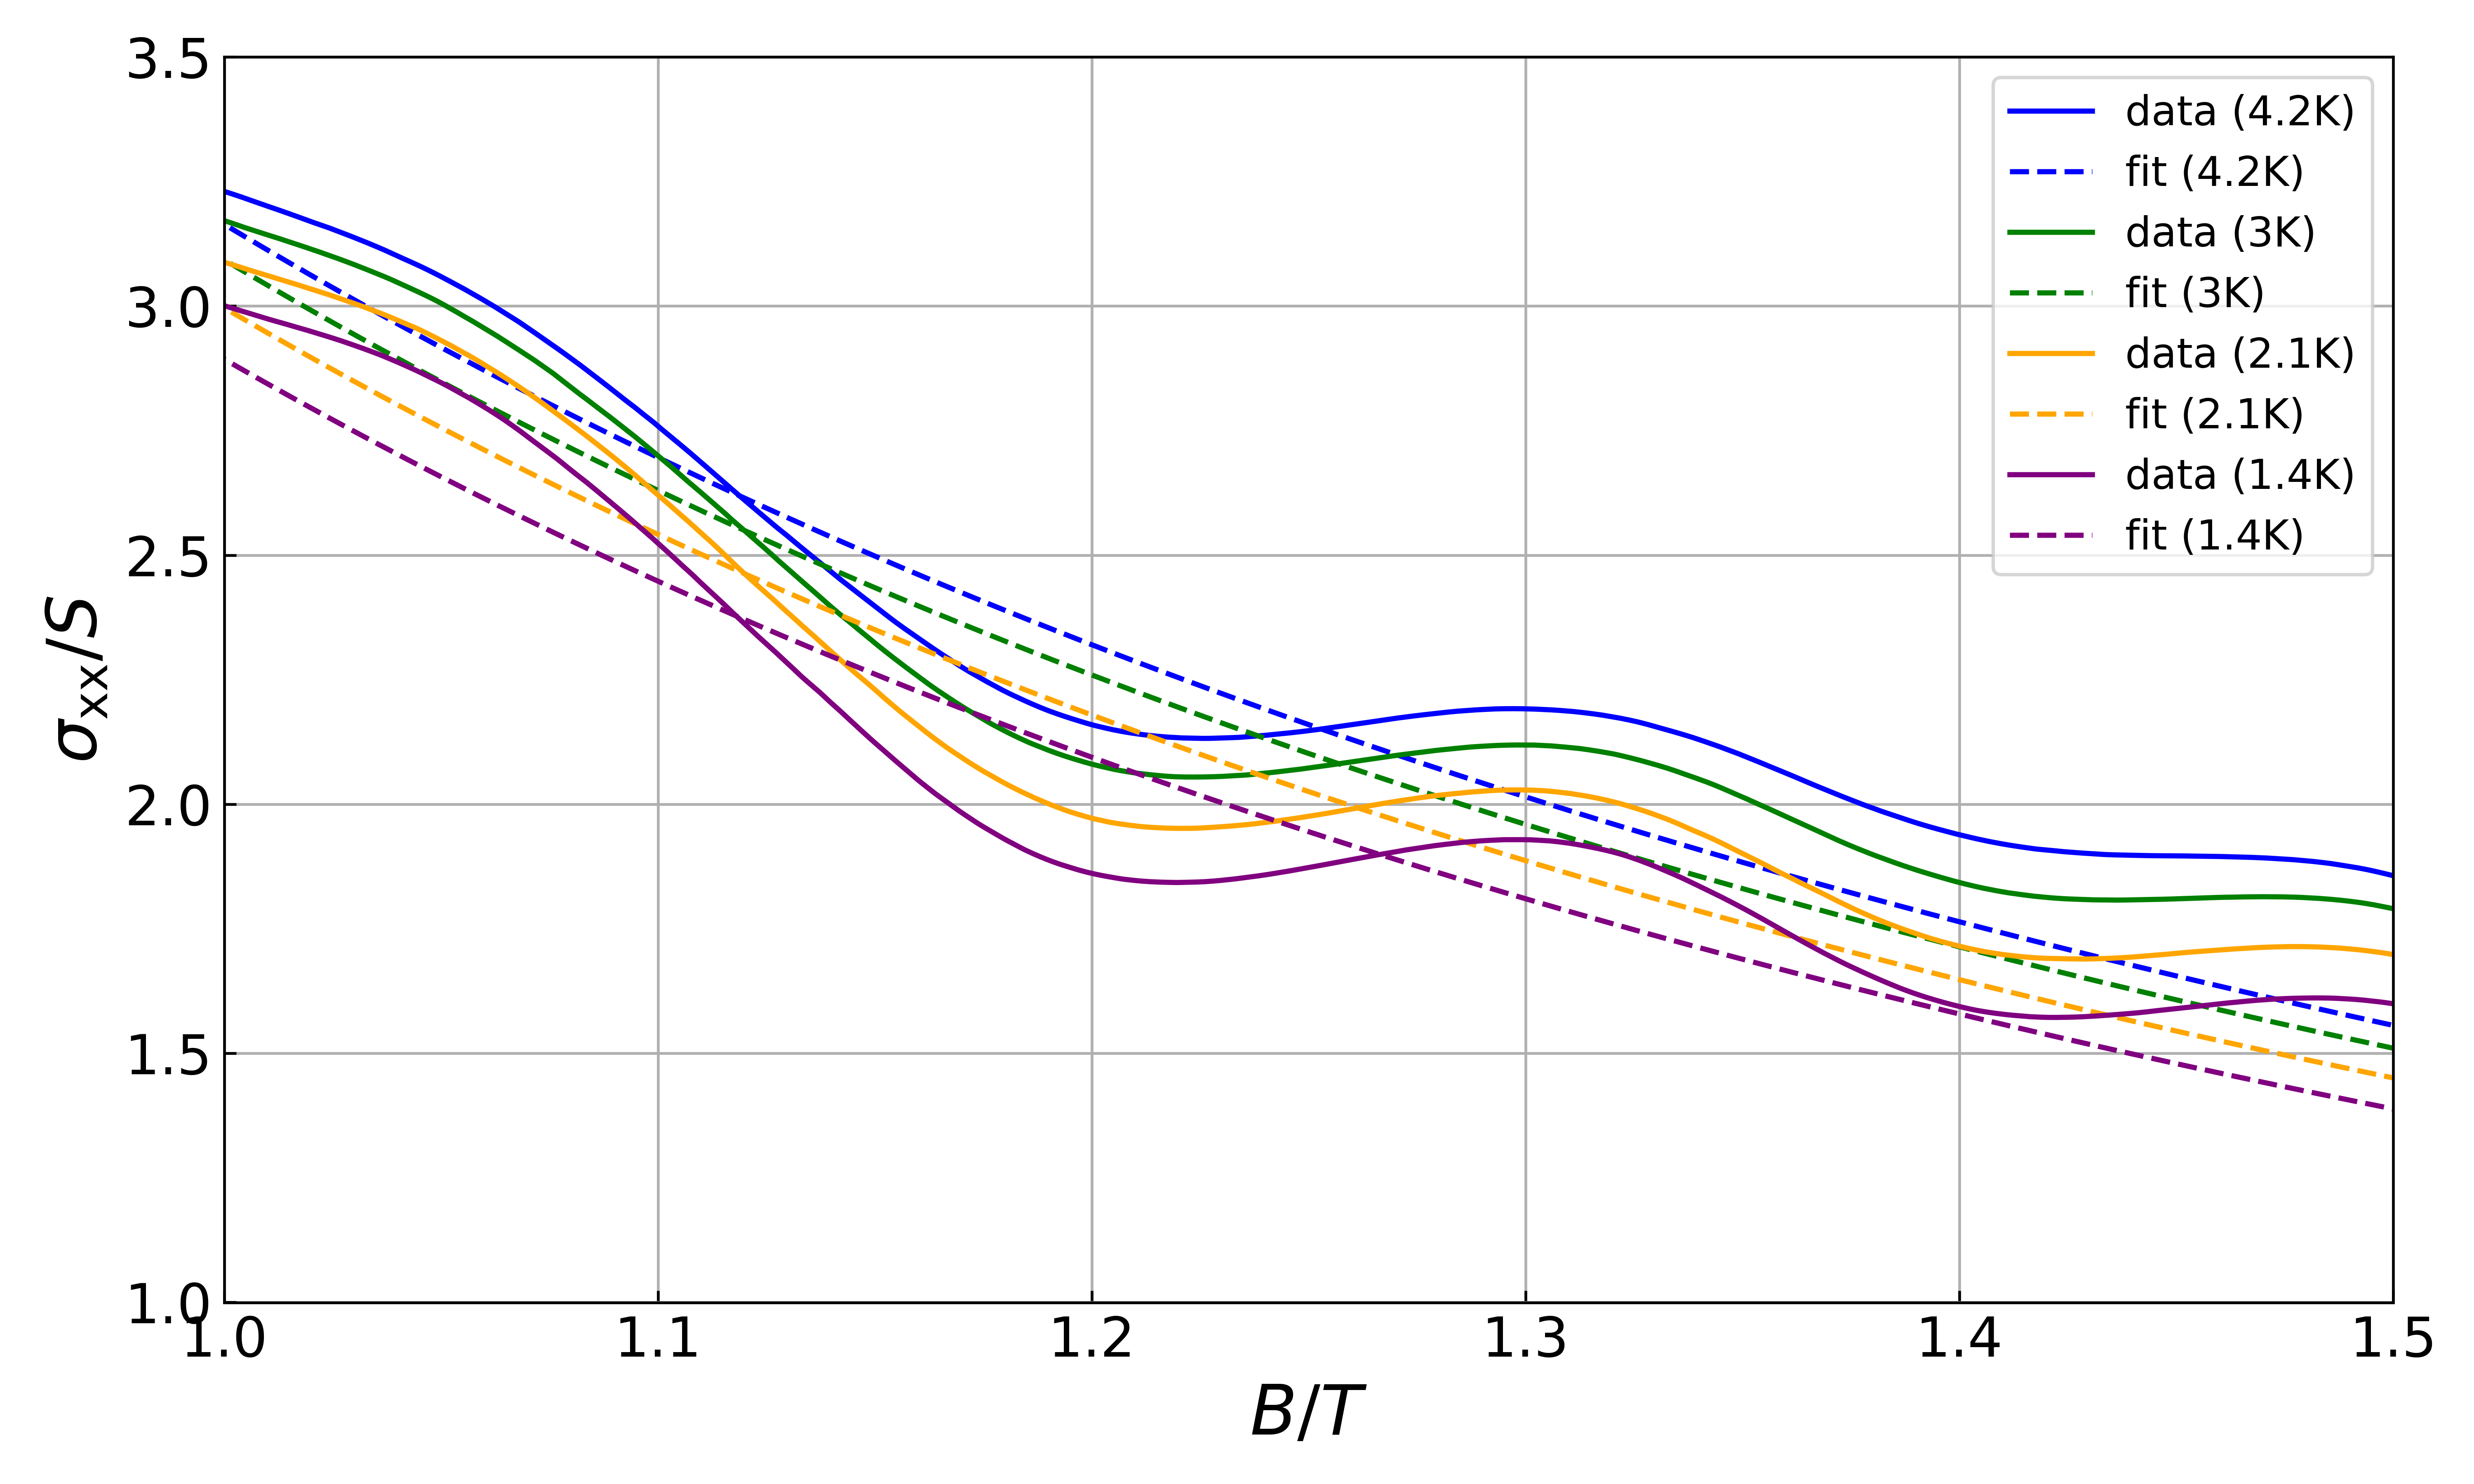
\includegraphics[width=0.45\textwidth]{../Images/sigmaWithFit.png}
    \caption{Examplary fit of the background of the longitudinal conductance $\sigma_\text{xx}$ at various temperatures. 
    The shown range of the plot is picked because of good visibility of the fit. The total fit is done for a wider range ($0.5\,\text{T}$ to $1.5\,\text{T}$) like stated in the text.}
    \label{fig:fitCyclotron}
\end{figure}
The fit is done for magnetic fields in the range $0.5\,\text{T}$ to $1.5\,\text{T}$, where the magnetic field is still small enough for eq.\,\ref{eq:sigmaxxCyclotron} to hold.
By dividing $\sigma_\text{xx}$ by $\sigma_\text{background}$ and adding a $1$, the oscillations can be isolated, as shown in fig.\,\ref{fig:oscillationsCyclotron}.
\begin{figure}[h]
    \centering
    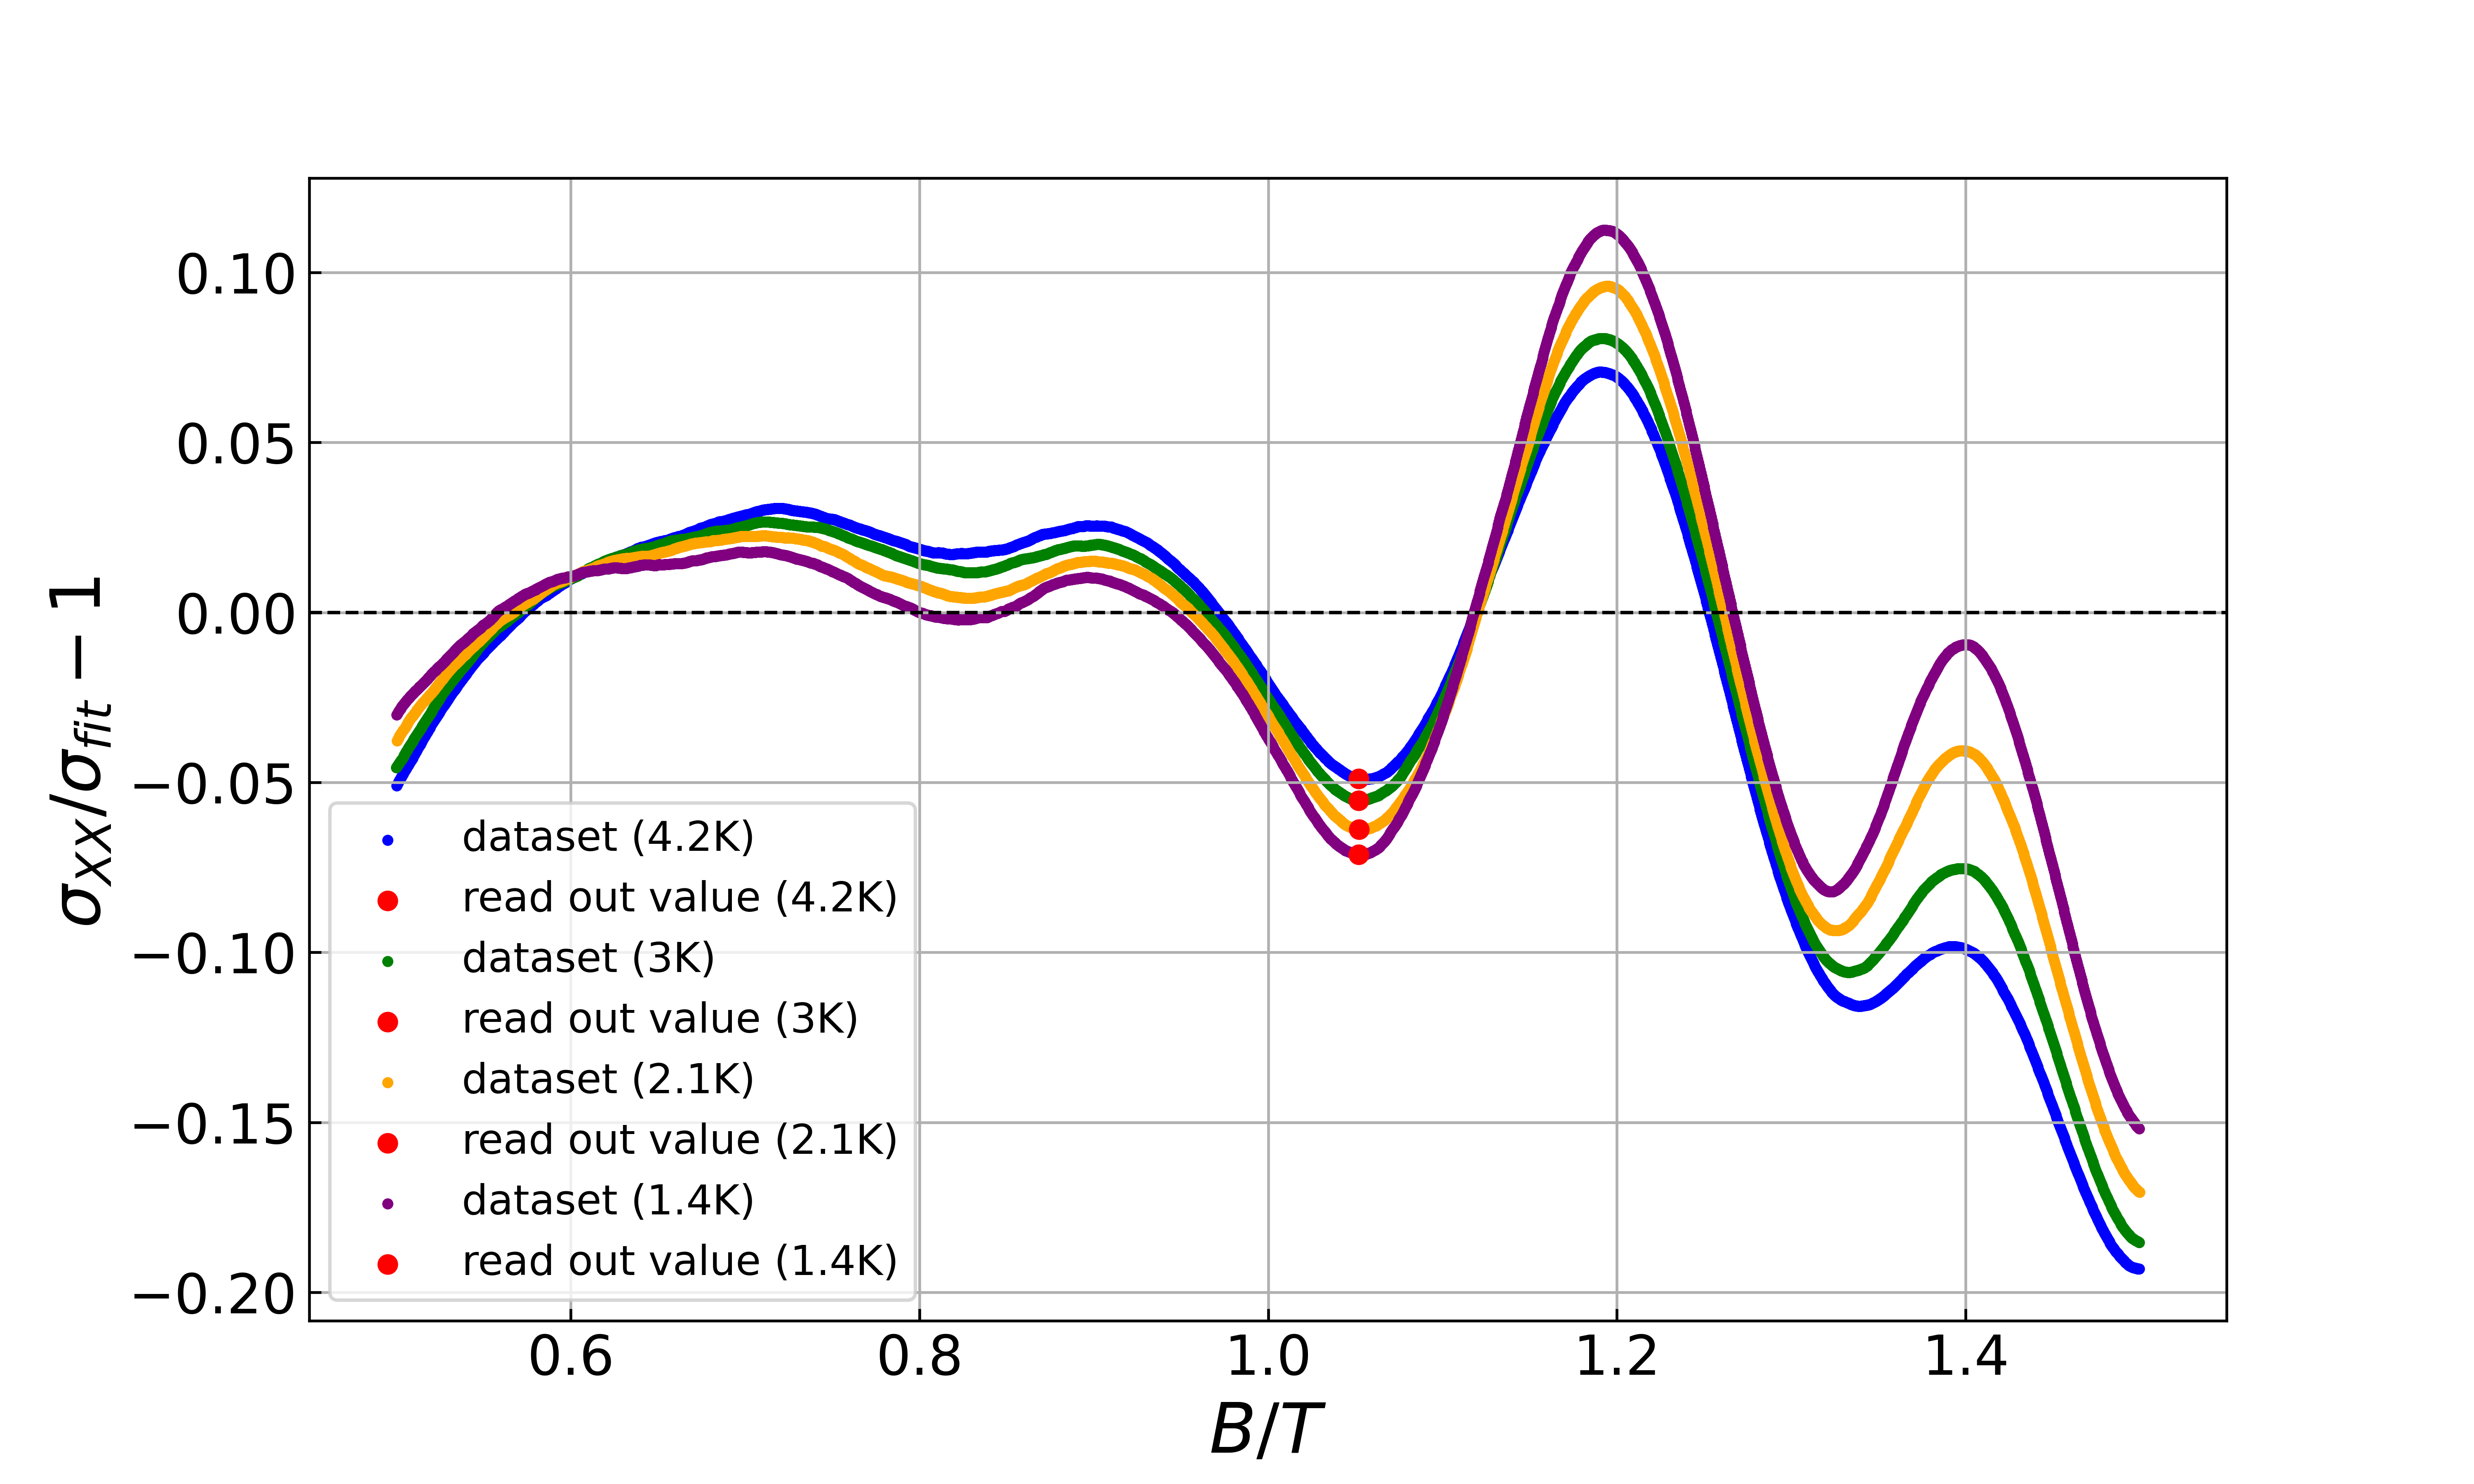
\includegraphics[width=0.45\textwidth]{../Images/reducedSigma.png}
    \caption{Isolated scillations of the longitudinal conductance $\sigma_\text{xx}$ at various temperatures.}
    \label{fig:oscillationsCyclotron}
\end{figure}
This is in accordance with eq.\,\ref{eq:sigmaxxCyclotron}, which then simplifies to eq.\,\ref{eq:onlyOscillation}
\begin{align}
    \sigma_\text{xx}(B) = A(B,T,\tau)\cdot\cos{\left(\frac{2\pi E_\text{F}}{\hbar\omega}\right)}
    \label{eq:onlyOscillation}
\end{align}
As shown in fig.\,\ref{eq:onlyOscillation}, the amplitudes of the first pronounced oscillation for the temperatures ($1.4\,K$,$3\,K$) and ($2.1\,K$,$4.2\,K$) are read out as pairs ($A(T_1)$,$A(T_2)$).
The chosen oscillation is small enough that $A_\text{ratio}=\frac{A(T_1)}{A(T_2)}$ eq.\,\ref{mc/me} is valid \cite{Tasksheet}.
\begin{align}
    \frac{m_\text{c}}{m_\text{e}}=\frac{\hbar eB}{m_\text{e}\pi^2k_\text{B}T_1}\text{arcosh}\left(A_\text{ratio}\right)\label{mc/me}
\end{align}
With eq.\,\ref{mc/me} the cyclotron mass $m_\text{c}$ can be calculated. The results are shown in tab.\,\ref{tab:cyclotronMass}.
\begin{table}[h]
    \centering
    \begin{tabular}{c|c}
        \hline\hline
        $m_{\text{c}1.4\text{K},3\text{K}}$ & $m_{\text{c}2.1\text{K},4.2\text{K}}$ \\\hline
        $(\csname cyclotron15\endcsname)\cdot 10^{-2}m_\text{e}$& $(\csname cyclotron21\endcsname)\cdot10^{-2}m_\text{e}$ \\
        \hline\hline
    \end{tabular}
    \caption{Calculated cyclotron masses for the pairs of temperatures. The values are given in units of the electron mass $m_\text{e}$. \label{tab:cyclotronMass}}
\end{table}
The literature expects cyclotron masses of $m_\text{c}= 0.026m_\text{e}$ to $m_\text{c}= 0.048m_\text{e}$ \cite{Xhang}.
The determined value for the pair $1.4\,K$ and $3\,K$ is in the range of the literature value, while the value for the pair $2.1\,K$ and $4.2\,K$ is slightly lower, but still agrees within its errors.
As can be seen in Fig.\,\ref{fig:oscillationsCyclotron}, the reading of the amplitude is very subjective and more error prone than the reading of the magnetic field.
In addition, some uncertainty in the background fit is included in the amplitude error.
On this basis, an error of $10\%$ is assumed for the amplitude and $1\%$ for the magnetic field.
The errors are calculated using Gaussian error propagation for the amplitude error and the corresponding magnetic field error.